Throughout the development of Yarn, acceptance tests and specifications were
written prior to developing a feature. This provided a solid test coverage
which in turn allowed for some radical refactorings to improve the quality,
readability and performance of the system. By the end of development, all
12 acceptance tests and 77 specifications passed. The final test coverage was
94.38\%, as depicted on Figure~\ref{coverage}. 

\begin{figure}[htb]
  \centering
  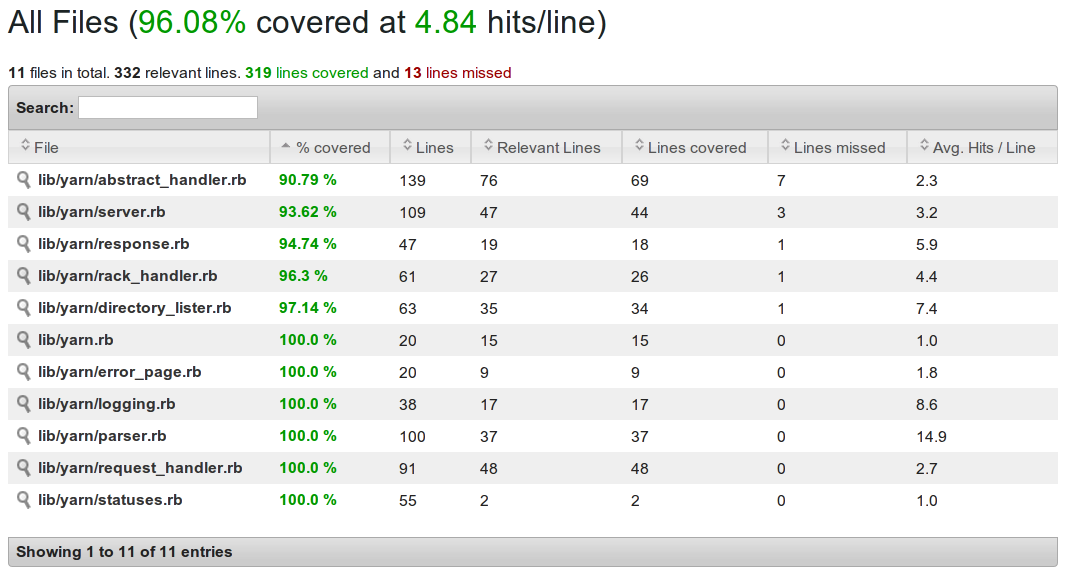
\includegraphics[width=1.0\textwidth]{img/coverage.png}
  \caption{Yarn test coverage screenshot.}
  \label{coverage}
\end{figure}

During the development, the test coverage was continously monitored to ensure
all parts of the system was exercised in the test suite. The test coverage
analysis is available on the CD in the \texttt{coverage} folder.

Some features were harder to test than others, and testing for concurrency was
especially tricky. The solution was to invoke two requests to a Ruby file
,which invoked the \texttt{sleep} method for a given amount of time before
returning the response. Firing a request which slept for a second would block
other requests from being served during that second. But if the server could
handle concurrent requests, a fast request fired after the slow request,
should be able to get it's response prior to the slow request completing.
Listing~\ref{confea} shows the acceptance test for concurrent requests.

\bigskip
\begin{lstlisting}[label=confea,caption=Concurrency acceptance test
(features/concurrency.feature:7)]
Scenario: Perform two requests in parallel
  Given the server is running
  Given a client "A"
  And a client "B"
  When client "A" makes a "1" second request
  And client "B" makes a "0.1" second request
  Then client "B" receives a response before client "A"
\end{lstlisting}

Having this acceptance test proved especially valuable during the
reimplementation of the concurrency feature from using threads to using
processes.
